\section{Base Theory and Concepts About Graphics}

\subsection{Image and Color Representation}

\begin{frame}{Light, pixels and pictures}
  \begin{itemize}
  \item Pictures are {\bf representations of light emissions}
  \item Analog representations are spatially {\bf continuous}:
    \begin{itemize}
    \item with an {\bf infinite} number of elements
    \item example : photosensitive paper
    \end{itemize}
  \item Digital representations are spatially {\bf quantified}:
    \begin{itemize}
    \item with a {\bf finite} number of elements
    \item example : discrete LED-based display
    \end{itemize}
  \item Producing a digital representation is called \textbf{quantization}
  \item Quantization requires a {\bf base element unit} or quantum
  \item This quantum is called picture element or {\bf pixel}
  \item Quantization is also called \textbf{sampling} in this context
  \end{itemize}
\end{frame}

\begin{frame}{Light, pixels and pictures}
  \begin{itemize}
  \item Quantified pixels have a \textbf{spatial density} or spatial resolution:\\
  \textit{How many pixels are found in \(n\) inches?}
  \item The usual pixel resolution unit is the \textbf{dot per inch} (DPI)
  \item Vertical and horizontal spatial densities are usually not distinguished
  \end{itemize}

  \begin{center}
  From single pixels to depicting a subject:
  \end{center}

  \begin{itemize}
  \item Pictures are bi-dimensional ordered ensembles of pixels (also called \textbf{frames})
  \item As such, pixels are disposed along two axis and each have a \textbf{position}:\\
   \textit{horizontal (\(x\)) and vertical (\(y\)) positions}
  \item Pictures have \textbf{dimensions}, expressed as a number of pixels:\\
   \textit{horizontal (\(width\)) and vertical (\(height\)) dimensions}
  \end{itemize}

\end{frame}

\begin{frame}{Light, pixels and pictures (illustrated)}
  \begin{minipage}[b]{0.45\textwidth}
    \centering
    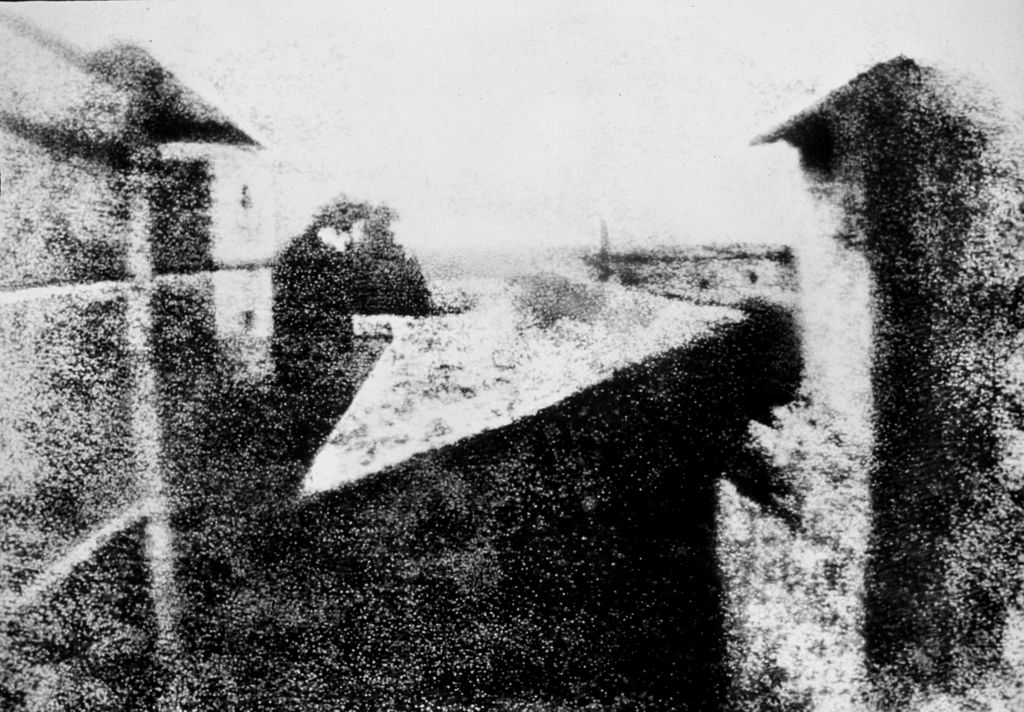
\includegraphics[width=\textwidth]{slides/graphics-theory/first-photo.jpg}
    \textit{\small View from the Window at Le Gras picture}
  \end{minipage}
  \hfill
  \begin{minipage}[b]{0.45\textwidth}
    \centering
    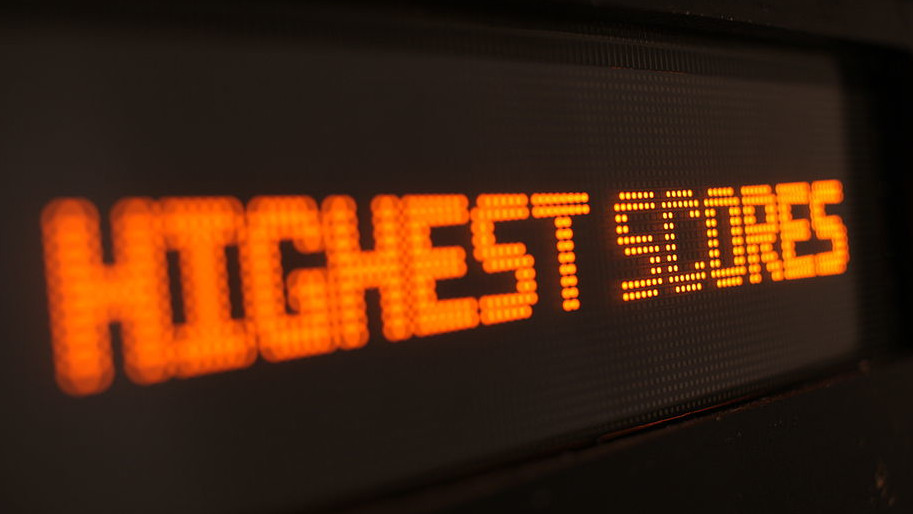
\includegraphics[width=\textwidth]{slides/graphics-theory/dot-matrix-display.jpg}
    \textit{\small A monochrome dot-matrix display}
  \end{minipage}

  \vspace{1em}

  \begin{minipage}[b]{0.45\textwidth}
    \centering
    \textbf{Analog representation},\\ on a metal plate
  \end{minipage}
  \hfill
  \begin{minipage}[b]{0.45\textwidth}
    \centering
    \textbf{Digital representation},\\ on a LED display
  \end{minipage}
\end{frame}

\begin{frame}{Sampling and frequency domain}
  \begin{itemize}
  \item Pixels are quantized/sampled representations of a \textbf{spatial domain}
  \item The initial (continuous) domain has a corresponding \textbf{frequency spectrum}\\
    \textit{high frequencies provide details in pictures}
  \item A 2D \textbf{Fourier transform} translates from spatial \((x,y)\) to frequency \((u,v)\) domain
\[
F(u,v) = \int_{-\infty}^{+\infty} \int_{-\infty}^{+\infty} f(x,y)e^{-j2\pi(ux+uy)}dxdy
\]
  \item Adapted for discrete signals as \textbf{Discrete Fourier Transform}
  \item Implemented with optimized algorithms as \textbf{Fast Fourier Transform} (FFT)
  \item \textbf{Frequency domain analysis} is very useful for signal treatment\\
    \textit{used at the roots of image compression}
  \end{itemize}
\end{frame}

\begin{frame}{Sampling and frequency domain (illustrated)}
  \begin{center}
  \begin{minipage}[b]{0.45\textwidth}
    \centering
    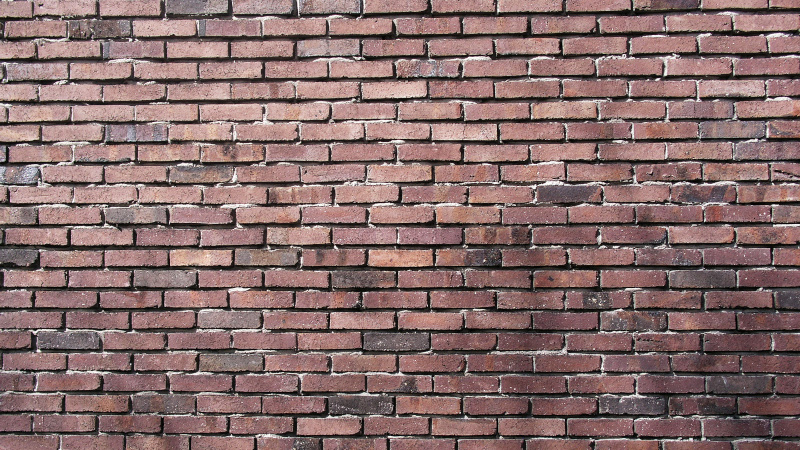
\includegraphics[width=\textwidth]{slides/graphics-theory/bricks.jpg}\\
    \textit{\small A wall of bricks represented in the spatial domain}
  \end{minipage}
  \hfill
  \begin{minipage}[b]{0.45\textwidth}
    \centering
    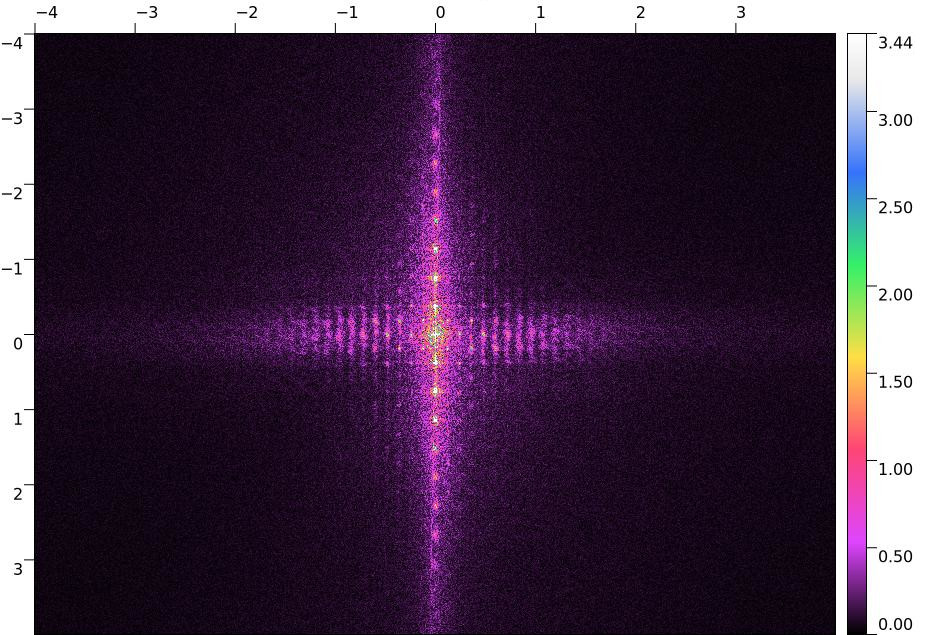
\includegraphics[width=\textwidth]{slides/graphics-theory/bricks-fft.jpg}\\
    \textit{\small The wall of bricks represented in the frequency domain}
  \end{minipage}

  \end{center}
\end{frame}

\begin{frame}{Sampling and frequency domain (illustrated)}
  \begin{minipage}[b]{0.45\textwidth}
    \centering
    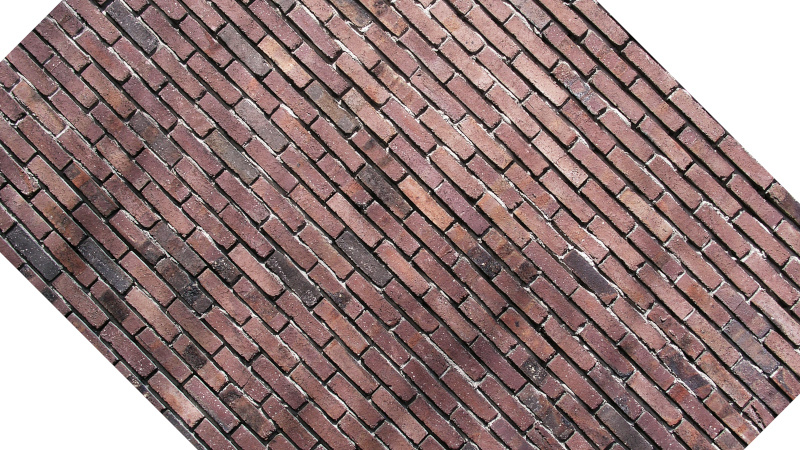
\includegraphics[width=\textwidth]{slides/graphics-theory/bricks-rotation.jpg}\\
    \textit{\small A wall of bricks rotated \(45^{\circ}\) represented in the spatial domain}
  \end{minipage}
  \hfill
  \begin{minipage}[b]{0.45\textwidth}
    \centering
    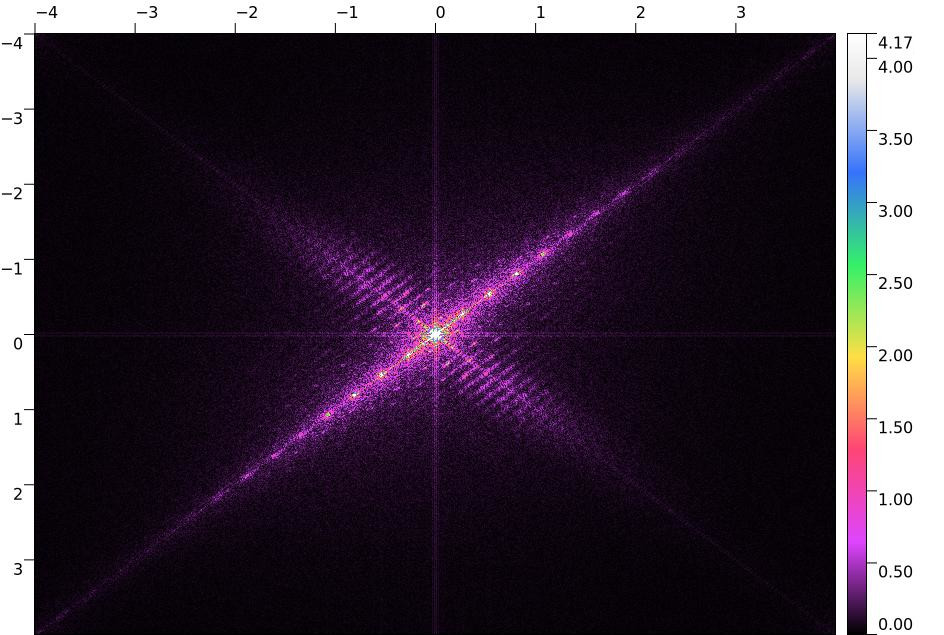
\includegraphics[width=\textwidth]{slides/graphics-theory/bricks-fft-rotation.jpg}\\
    \textit{\small The wall of bricks rotated \(45^{\circ}\) represented in the frequency domain}
  \end{minipage}
\end{frame}

\begin{frame}{Sampling and aliasing}
  \begin{itemize}
  \item The spatial domain is quantized with a bi-dimensional \textbf{sampling resolution}
  \item Matching \textbf{sampling frequencies} exist, for each axis: \((u_s,v_s)\)
  \item They \textbf{limit the frequencies} that can be sampled from the initial domain
  \item The \textbf{Shanon-Nyquist theorem} provides a sufficient condition for \((u_s,v_s)\):
\[
u_s > 2 \times u_max, ~v_s = 2 \times v_{max}
\]
  \item Frequencies such that \(f \geq \frac{u_s}{2}\) are \textbf{not correctly sampled}
  \item Results in \textbf{incorrect frequencies} being introduced: \textbf{Moiré pattern} in 2D
  \end{itemize}

  \begin{center}
  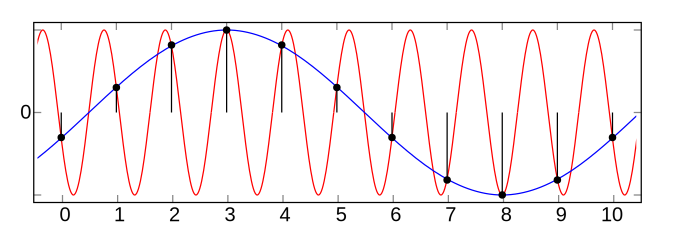
\includegraphics[width=0.35\textwidth]{slides/graphics-theory/aliasing-1d.pdf}\\
  \textit{\small Aliasing in a uni-dimensional domain}
  \end{center}
\end{frame}

\begin{frame}{Sampling and aliasing (illustrated)}
  \begin{minipage}[b]{0.29\textwidth}
    \centering
    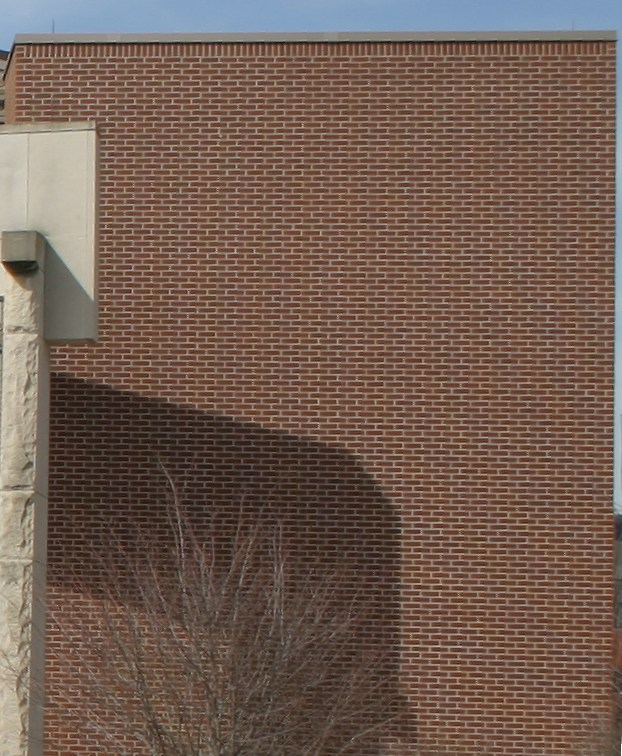
\includegraphics[width=\textwidth]{slides/graphics-theory/bricks-rich.jpg}\\
    \textit{\small Another wall of bricks}
  \end{minipage}
  \hfill
  \begin{minipage}[b]{0.29\textwidth}
    \centering
    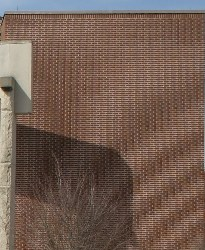
\includegraphics[width=\textwidth]{slides/graphics-theory/bricks-alias.jpg}\\
    \textit{\small Moiré on the bricks}
  \end{minipage}
  \hfill
  \begin{minipage}[b]{0.29\textwidth}
    \centering
    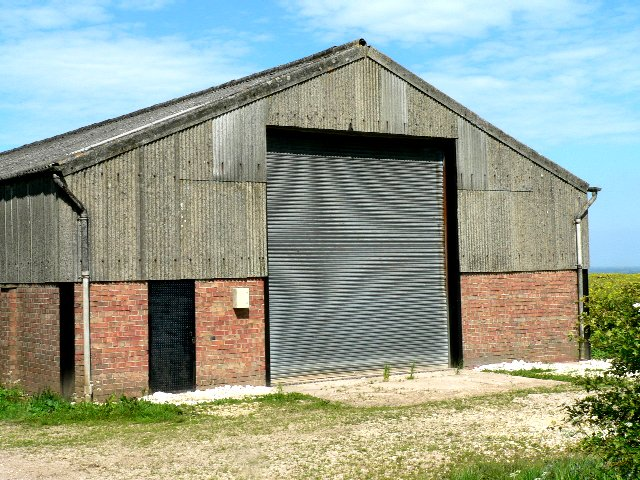
\includegraphics[width=\textwidth]{slides/graphics-theory/moire.jpg}\\
    \textit{\small Moiré on the garage door}
  \end{minipage}
\end{frame}

\begin{frame}{Light representation, color quantization}
  \begin{minipage}[c]{0.75\textwidth}
    \begin{itemize}
    \item Light itself must be quantized in digital representations\\
    \textit{distinct from and unrelated to spatial quantization}
    \item Translating light information (colors) to numbers
    \item The translation referential is called \textbf{colorspace}
    \item The translated color has coordinates in the colorspace\\
    \textit{e.g. 3 for a human-eye-alike referential: red, green, blue}
    \item The color coordinates are quantized with:
      \begin{itemize}
      \item A given \textbf{resolution}:
      \textit{the smallest possible color difference}
      \item A given \textbf{range}:
      \textit{the span of representable colors}
      \end{itemize}
    \item Both aspects of color quantization depend on:
      \begin{itemize}
      \item The colorspace taken as referential
      \item The color depth or number of \textbf{bits per pixel} (bpp)
      \item Implementation choices
      \end{itemize}
    \end{itemize}
  \end{minipage}
  \hfill
  \begin{minipage}[c]{0.225\textwidth}
    \centering
    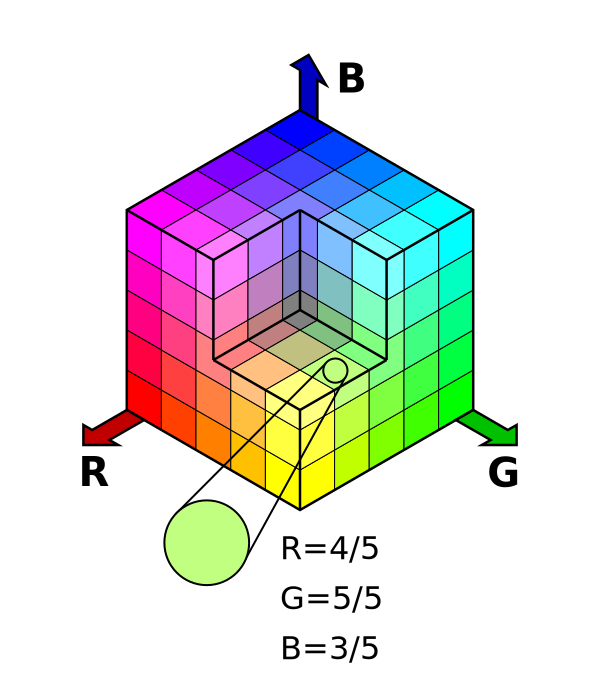
\includegraphics[width=\textwidth]{slides/graphics-theory/rgb-cube.pdf}
  \end{minipage}
\end{frame}

\begin{frame}{Light representation, color quantization (illustrated)}
  \begin{minipage}[b]{0.45\textwidth}
    \centering
    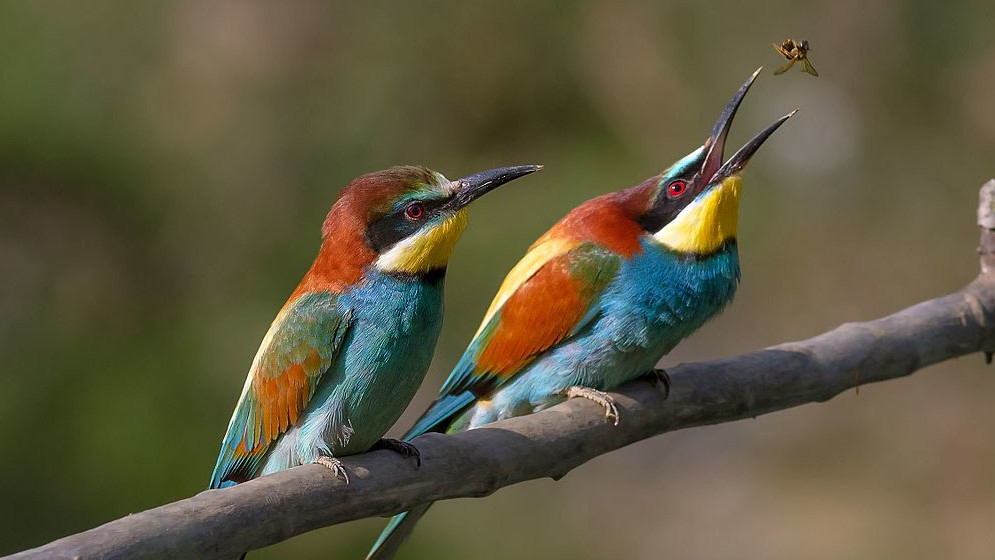
\includegraphics[width=\textwidth]{slides/graphics-theory/pair-of-merops.jpg}
  \end{minipage}
  \hfill
  \begin{minipage}[b]{0.45\textwidth}
    \centering
    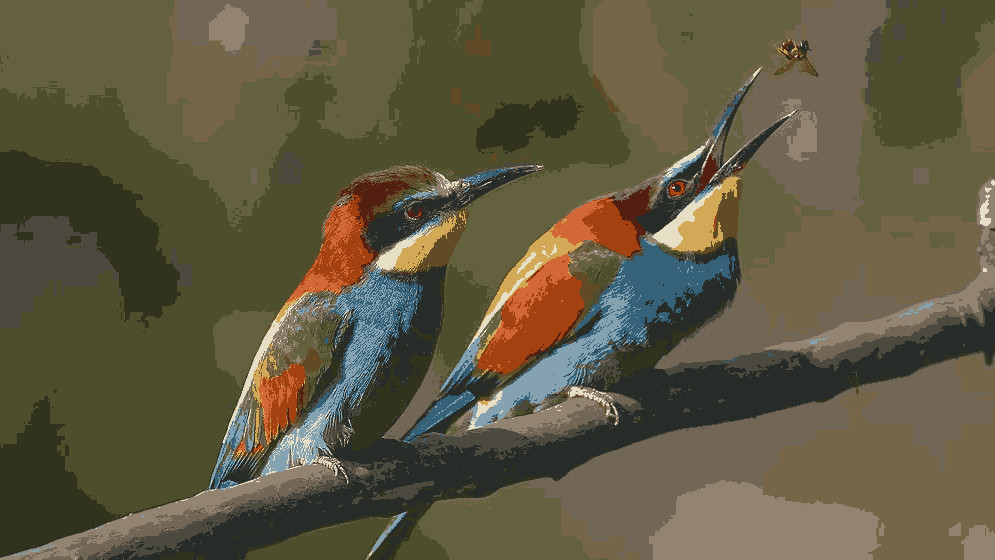
\includegraphics[width=\textwidth]{slides/graphics-theory/pair-of-merops-16-colors.jpg}
  \end{minipage}

  \begin{center}
     \textit{\small A pair of Merops feeding}
  \end{center}

  \begin{minipage}[b]{0.45\textwidth}
    \centering
    \textbf{16 million colors (24 bits per pixel)}
    \begin{itemize}
    \item high color resolution
    \item high color range
    \end{itemize}
  \end{minipage}
  \hfill
  \begin{minipage}[b]{0.45\textwidth}
    \centering
    \textbf{16 colors (4 bits per pixel)}
    \begin{itemize}
    \item low color resolution
    \item low color range
    \end{itemize}
  \end{minipage}
\end{frame}

\begin{frame}{Light representation, color quantization (illustrated)}
  \begin{minipage}[b]{0.45\textwidth}
    \centering
    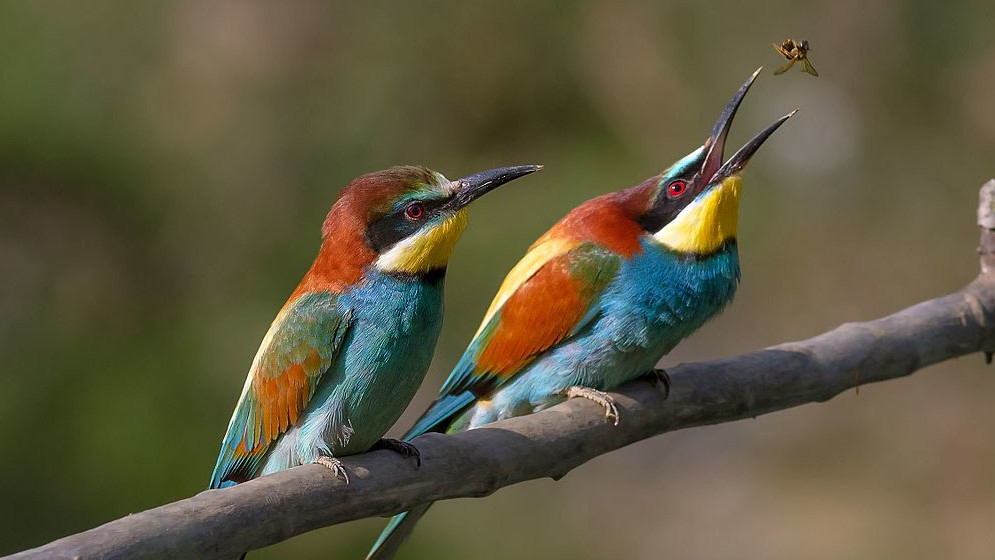
\includegraphics[width=\textwidth]{slides/graphics-theory/pair-of-merops.jpg}
  \end{minipage}
  \hfill
  \begin{minipage}[b]{0.45\textwidth}
    \centering
    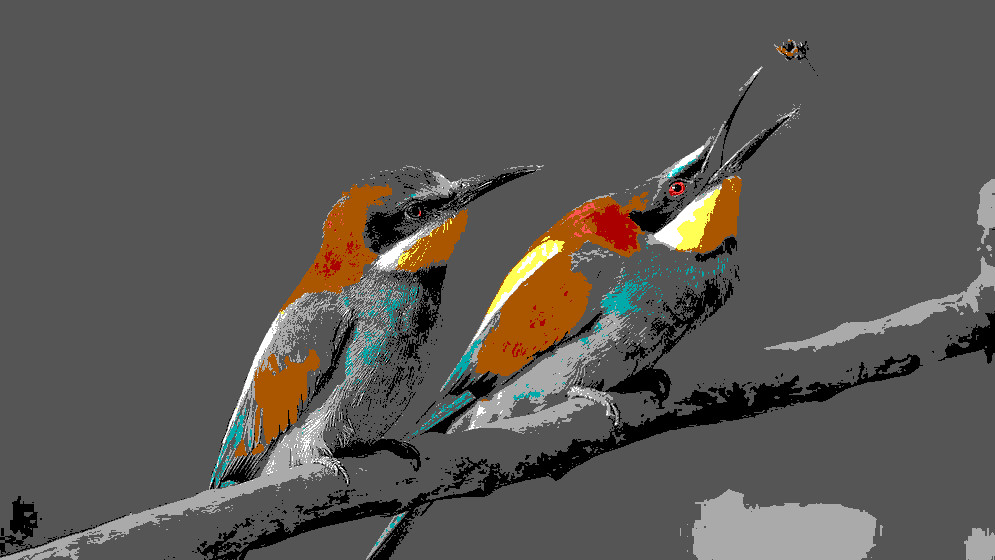
\includegraphics[width=\textwidth]{slides/graphics-theory/pair-of-merops-16-colors-range.jpg}
  \end{minipage}

  \begin{center}
     \textit{\small A pair of Merops feeding}
  \end{center}

  \begin{minipage}[b]{0.45\textwidth}
    \centering
    \textbf{16 million colors (24 bits per pixel)}
    \begin{itemize}
    \item high color resolution
    \item high color range
    \end{itemize}
  \end{minipage}
  \hfill
  \begin{minipage}[b]{0.45\textwidth}
    \centering
    \textbf{16 colors (4 bits per pixel)}
    \begin{itemize}
    \item lower color resolution
    \item high color range
    \end{itemize}
  \end{minipage}
\end{frame}

\begin{frame}{Level of detail of quantized pictures}
  Depends on a number of factors, including:
  \begin{itemize}
  \item Spatial density (pixel resolution)
  \item Quantized dimensions (picture width and height)
  \item Colorspace limits (chromaticity diagram)
  \item Color depth (number of bits per pixel)
  \item Color resolution and range trade-off
  \end{itemize}~

  Generally speaking:
  \begin{itemize}
  \item Many factors are involved
  \item The major bottleneck is not always obvious
  \item Implementation choices do matter
  \end{itemize}
\end{frame}

\begin{frame}{Colorspaces and channels}
  \begin{minipage}[b]{0.7\textwidth}
    \begin{itemize}
    \item Each component of a colorspace is called a \textbf{channel}
    \item Examples for usual types of colorspaces:
      \begin{itemize}
      \item RGB, with 3 channels:\\ \textbf{R} (red) / \textbf{G} (green) / \textbf{B} (blue)
      \item HSV, with 3 channels:\\ \textbf{H} (hue) / \textbf{S} (saturation) / \textbf{V} (value)
      \item YUV or Y/Cb/Cr, with 3 channels:\\ \textbf{Y} (luminance) / \textbf{U or Cb} / \textbf{V or Cr} (chrominance)
      \end{itemize}
    \end{itemize}
  \end{minipage}
  \hfill
  \begin{minipage}[b]{0.25\textwidth}
    \centering
    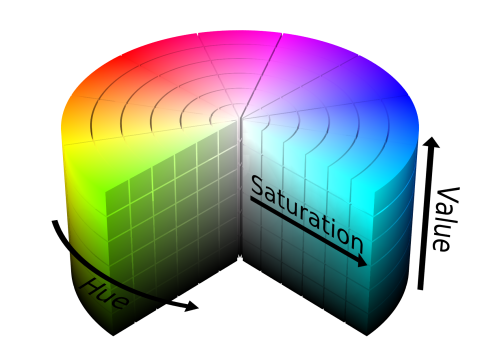
\includegraphics[width=\textwidth]{slides/graphics-theory/hsv-diagram.pdf}\\
    \vspace{-1em}
    \textit{\small HSV diagram}
    \vspace{0.25em}
  \end{minipage}
  \begin{itemize}
  \item An additional channel can exist for transparency: the \textbf{alpha channel}\\
  \textit{mostly relevant for composition, not for final display}
  \item Color coordinates can be \textbf{converted} from one colorspace to another (CSC)\\
  \textit{using translation formulas and associated constants}
  \end{itemize}
\end{frame}

\begin{frame}{Colorspaces and channels (illustrated with YUV)}
  \begin{minipage}[t]{0.25\textwidth}
    \centering
    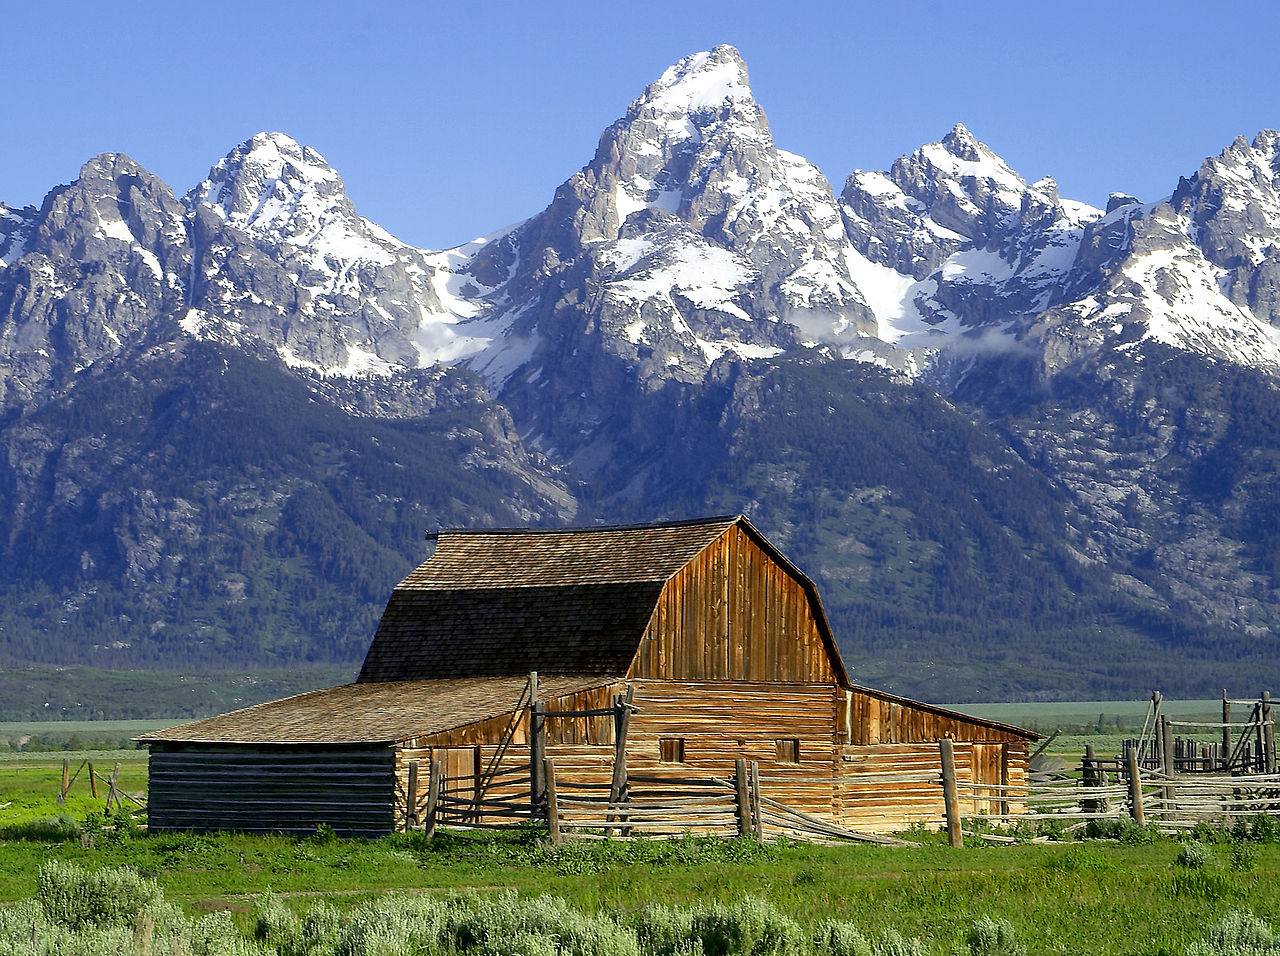
\includegraphics[height=6em]{slides/graphics-theory/barn.jpg}\\
    \textit{\small Original picture}
  \end{minipage}
  \hfill
  \begin{minipage}[t]{0.7\textwidth}
    \centering
    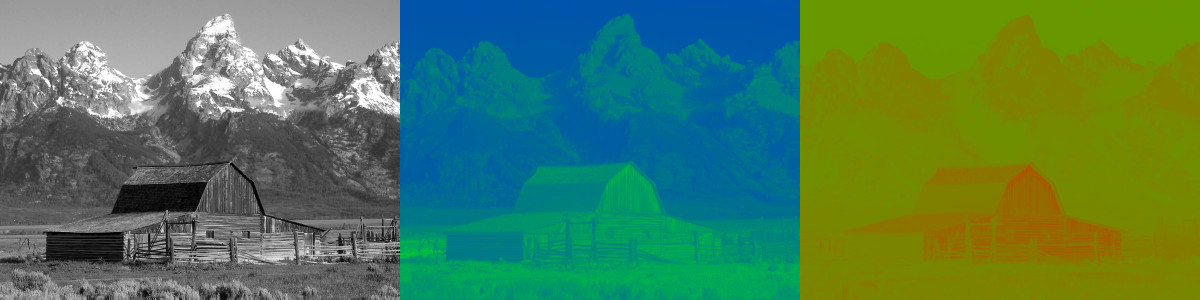
\includegraphics[height=6em]{slides/graphics-theory/barn-yuv.jpg}\\
    \textit{\small Decomposition in Y, U and V channels}
  \end{minipage}

  \vspace{1em}

  \begin{minipage}[t]{0.4\textwidth}
    \small
    \begin{equation*}
    \begin{cases}
    R = Y + 1.140 \times V\\
    G = Y - 0.395 \times U - 0.581 \times V\\
    B = Y + 2.032 \times U
    \end{cases}
    \end{equation*}
  \end{minipage}
  \hfill
  \begin{minipage}[t]{0.55\textwidth}
    \small
    \begin{equation*}
    \begin{cases}
    Y = + 0.299 \times R + 0.587 \times G + 0.114 \times B\\
    U = - 0.147 \times R - 0.289 \times G + 0.436 \times B\\
    V = + 0.615 \times R - 0.515 \times G - 0.100 \times B
    \end{cases}
    \end{equation*}
  \end{minipage}

  \begin{center}
     \textit{\small Translation between BT.609 YUV and sRGB colorspaces}
  \end{center}
\end{frame}

\begin{frame}{Frame size and chroma sub-sampling}
  \begin{itemize}
  \item Digital pictures easily take up a lot of space (moreso for videos)
  \item The minimal size for a picture depends on:
    \begin{itemize}
    \item Dimensions (\(width\) and \(height\))
    \item Color (and alpha) depth or bits per pixel (\(bpp\))
    \item Roughly: \(width \times height \times bpp \div 8~bytes\)
    \item For 12 Mpixels with 16 Mcolors and alpha: \(4000 \times 3000 \times 32 \div 8 = 45.8 MiB\)
    \end{itemize}
  \item The human visual system has specificities:
    \begin{itemize}
    \item High sensitivity to \textbf{luminosity} (luminance)
    \item Low sensibility to \textbf{colors} (chrominance)
    \end{itemize}
  \item YUV colorspaces offer the relevant channel separation
  \item Sub-sampling can be applied to the chrominance channel\\
  \textit{less data (and precision) on colors to reduce size}
  \end{itemize}
\end{frame}

\begin{frame}{Frame size and chroma sub-sampling}
  \begin{itemize}
  \item Chrominance samples are used for multiple luminance samples
  \item With specific vertical and horizontal ratios (usually integer)
  \item Usually summarized using a three-part ratio: \(J:a:b\)
  \end{itemize}

  \begin{center}
  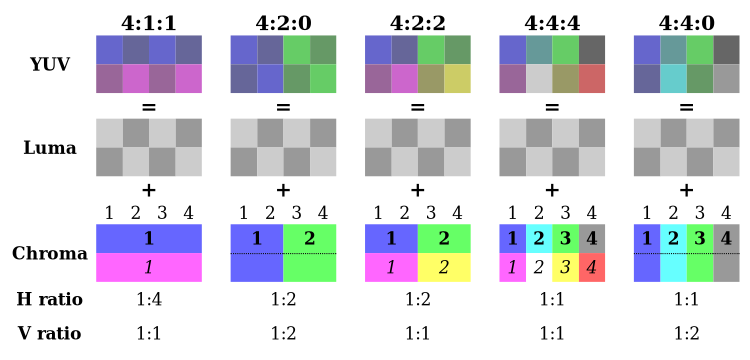
\includegraphics[width=0.7\textwidth]{slides/graphics-theory/yuv-sub-sampling.pdf}

  YUV 4:2:0 usual example:\\
  {\small\(bpp_Y = 8,~bpp_U = 8 / 2 = 4,~bpp_V = 8 / 2 = 4 ~\Rightarrow~ bpp = 16~bits/pixel\)}
  \end{center}
\end{frame}

\begin{frame}{Pixel data distribution in memory}
  \begin{itemize}
  \item Pixel data can be \textbf{distributed} in different ways in memory
  \item Different ways to aggregate color components in \textbf{data planes} (memory chunks):
    \begin{itemize}
    \item \textbf{Packed}: Components are stored in the same data plane in memory
    \item \textbf{Semi-planar} (YUV): Luma and chroma are stored in distinct data planes
    \item \textbf{Planar}: Each component has its own data plane in memory
    \end{itemize}
  \item When multiple color components are grouped, \textbf{bit order} must be specified:
    \begin{itemize}
    \item Which component comes first in memory?
    \item Affected by endianness when read by hardware!
    \end{itemize}
  \item \textbf{Scan order} must also be specified:
    \begin{itemize}
    \item How to calculate the address for position \((x,y)\) and back?
    \item Raster order (most common) specifies: row-major, left-to-right, top-to-bottom
    \end{itemize}
  \end{itemize}
  \begin{center}
  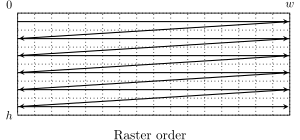
\includegraphics[height=6em]{slides/graphics-theory/raster-order.pdf}
  \end{center}
\end{frame}

\begin{frame}[fragile]{Pixel formats, FourCC codes}
  \begin{itemize}
  \item Many meta-data elements are needed to fully describe how a picture is coded
    \begin{itemize}
    \item Some describe \textbf{picture-level attributes} (e.g. dimensions)
    \item Some describe \textbf{pixel-level attributes} (e.g. colorspace, bpp)
    \end{itemize}
  \item Pixel-level attributes are grouped as a \textbf{pixel format} that defines:
    \begin{itemize}
    \item Colorspace in use
    \item Number of bits per channel and per pixel (bpp)
    \item Bit attribution and byte order
    \item Per-channel sub-sampling ratios
    \item Pixel data planes distribution in memory
    \end{itemize}
  \item Often represented as a 4-character code called \textbf{FourCC} {\small(\url{https://fourcc.org/})}
  \item Not really standardized and implementation-specific:\\
    \textit{DRM in Linux uses \code{XR24}, for \code{DRM_FORMAT_XRGB8888}}
  \textit{Not really standardized but widely used in various forms}
  \item Scan order is specified separately with a \textbf{modifier}\\
    \textit{assumed to be raster order if unspecified}
  \end{itemize}
\end{frame}

\subsection{Pixel Drawing}

\begin{frame}{Accessing pixel data}
  \begin{itemize}
  \item Pixel data is stored in memory, with a base address
  \item CPU access is either byte or word-aligned
    \begin{itemize}
    \item Good fit for formats with \(bpp = 32\) (very common)
    \item Good fit for formats with \(bpp = 8 \times n\)
    \item Not always easy to manage otherwise
    \end{itemize}
  \item The size of each line is called \textbf{stride} or \textbf{pitch}
    \begin{itemize}
    \item Usually equals: \(stride = width \times bpp \div 8\)
    \item Can contain an extra dead zone at the end
    \item Needs to be specified explicitly
    \end{itemize}
  \item The address of a pixel at \((x,y)\) in raster order is:
\[
address = address_{base} + y \times stride + x \times bpp \div 8
\]
  \end{itemize}
\end{frame}

\begin{frame}[fragile]{Iterating over pixel data}
  \begin{itemize}
  \item Pixel data can be access by iterating nested variables:
  \begin{minted}[fontsize=\small]{c}
for (y = 0; y < height; y++)
  for (x = 0; x < width; x++)
    data = base + y * stride + x * bpp / 8;
  \end{minted}
  \item Iterating over all pixels takes numerous CPU-cycles, tips:
    \begin{itemize}
    \item Incrementing the address instead of re-calculating it:
  \begin{minted}[fontsize=\small]{c}
data = base;
for (y = 0; y < height; y++)
  for (x = 0; x < width; x++)
    data += bpp / 8;
  data += stride - width * 8 / bpp;
  \end{minted}
    \item Iterating in y-major is also better for cache hits
    \item Beware: C pointer arithmetic uses type size as unit
    \end{itemize}
  \end{itemize}
\end{frame}

\begin{frame}{Rectangle drawing}
  \begin{itemize}
  \item A rectangle is defined with two boundaries par axis:
\[
x_{min} \leq x \leq x_{max},~ y_{min} \leq y \leq y_{max}
\]
  \item Another expression involves a (top-left) start point and size:
\[
x_{start} \leq x \leq x_{start} + x_{size},~ y_{start} \leq y \leq y_{start} + y_{size}
\]
  \item Allows iterating in the rectangle area only
  \end{itemize}
\end{frame}

\begin{frame}{Linear gradient drawing}
  \begin{itemize}
  \item Same base as drawing a rectangle
  \item A linear gradient involves interpolation between two colors
  \item Following one of the two axis as major
  \item Involves weighting the two colors depending on the advancement
  \item Equations in x-axis major:
  \end{itemize}
\begin{align*}
r &= r_{start} + (r_{stop} - r_{start}) \frac{x - x_{start}}{x_{size}}\\
g &= g_{start} + (g_{stop} - g_{start}) \frac{x - x_{start}}{x_{size}}\\
b &= b_{start} + (b_{stop} - b_{start}) \frac{x - x_{start}}{x_{size}}
\end{align*}
\end{frame}

\begin{frame}{Disk drawing}
  \begin{itemize}
  \item A disk is delimited with a radius test (\((0,0)\)-centered):
\[
\sqrt{x^2 + y^2} \leq radius
\]
  \item Given a center point \((x_c,y_c)\):
\[
\sqrt{(x - x_c)^2 + (y - y_c)^2} \leq radius
\]
  \item Requires iterating in:
\[
x_c - radius \leq x \leq x_c + radius,~ y_c - radius \leq y \leq y_c + radius
\]
  \end{itemize}
\end{frame}

\begin{frame}{Circular gradient drawing}
  \begin{itemize}
  \item Same base as drawing a disk
  \item Interpolation between two colors using the radius as major:
  \end{itemize}
\begin{align*}
d &= \sqrt{(x - x_c)^2 + (y - y_c)^2}\\
r &= r_{start} + (r_{stop} - r_{start}) \frac{d}{radius}\\
g &= g_{start} + (g_{stop} - g_{start}) \frac{d}{radius}\\
b &= b_{start} + (b_{stop} - b_{start}) \frac{d}{radius}
\end{align*}
\end{frame}


\subsection{Pixel Operations}

